\subsection{Electronic Circuits}
\subsubsection{Basic Concepts}
\begin{enumerate}
    \item Voltage \& Current divider Rule\\
    \begin{circuitikz} [american]
        \draw
        (0,0)
            to[V, l=$V(t)$] (0,3)
            to[R, l=$Z_1$, v<=$V_1(t)$, i>^=$i(t)$] (3,3) % The voltage source and resistor Z1
            to[short, -*] (4,3)
            to[R, l=$Z_2$, i>^=$i_1(t)$] (4,0) % The resistor Z2
            to[short, -*] (3,0)
        (4,3) 
            to[short] (6,3)
            to[R, l=$Z_3$, v<=$V_3(t)$, i<=$i_2(t)$] (6,0) % The resistor Z3
            to[short] (4,0)
        (3,3) 
            to[open, v^>=$V_2(t)$] (3,0) % The open circuit for voltage V2(t)
        (0,0) 
            to[short] (6,0)
        ;
        \draw [dashed] (2.5,3.5) rectangle (7.0,-0.5) node[above right] {$Z_{\text{Total}}$};
        \draw (3,-1) node {$\frac{1}{Z_{\text{Total}}} = \frac{1}{Z_2} + \frac{1}{Z_3}$};
    \end{circuitikz}\\
    For Voltages:
    \begin{align*}
        V(t) &= V_1(t) + V_2(t) \\
        V_1(t) &= \frac{Z_1(t)}{Z_1(t) + Z_{\text{Total}}(t)} V(t) \\
        V_2(t) &= \frac{Z_{\text{Total}}(t)}{Z_1(t) + Z_{\text{Total}}(t)} V(t)
    \end{align*}
    For Currents:
    \begin{align*}
    I(t) &= I_1(t) + I_2(t) \\
    I_1(t) &= \frac{Z_3(t)}{Z_2(t) + Z_3(t)} I(t) \\
    I_2(t) &= \frac{Z_2(t)}{Z_2(t) + Z_3(t)} I(t)
    \end{align*}
    \item Node Analysis KCL
    \begin{center}
    \begin{circuitikz}[american]
    \draw(0,1) to [short, -*, i=$i_y$](0,0);
    \draw(-1,0) to [short, -*, i=$i_x$](0,0);
    \draw (1,0) to [short, -*, i=$i_z$](0,0);
    \end{circuitikz}
    \end{center}
    Currents flowing into a network sum to zero. Since current $i$ is equal to the rate of flow of charge $q$ that $i = \frac{dq}{dt}$, KCL corresponds to the conservation of charge. You can view KCL as a netwrok, and all currents flow into the network sums to zero.\\
    \begin{exam}
    $\;$
    \begin{figure}[h]
        \centering
        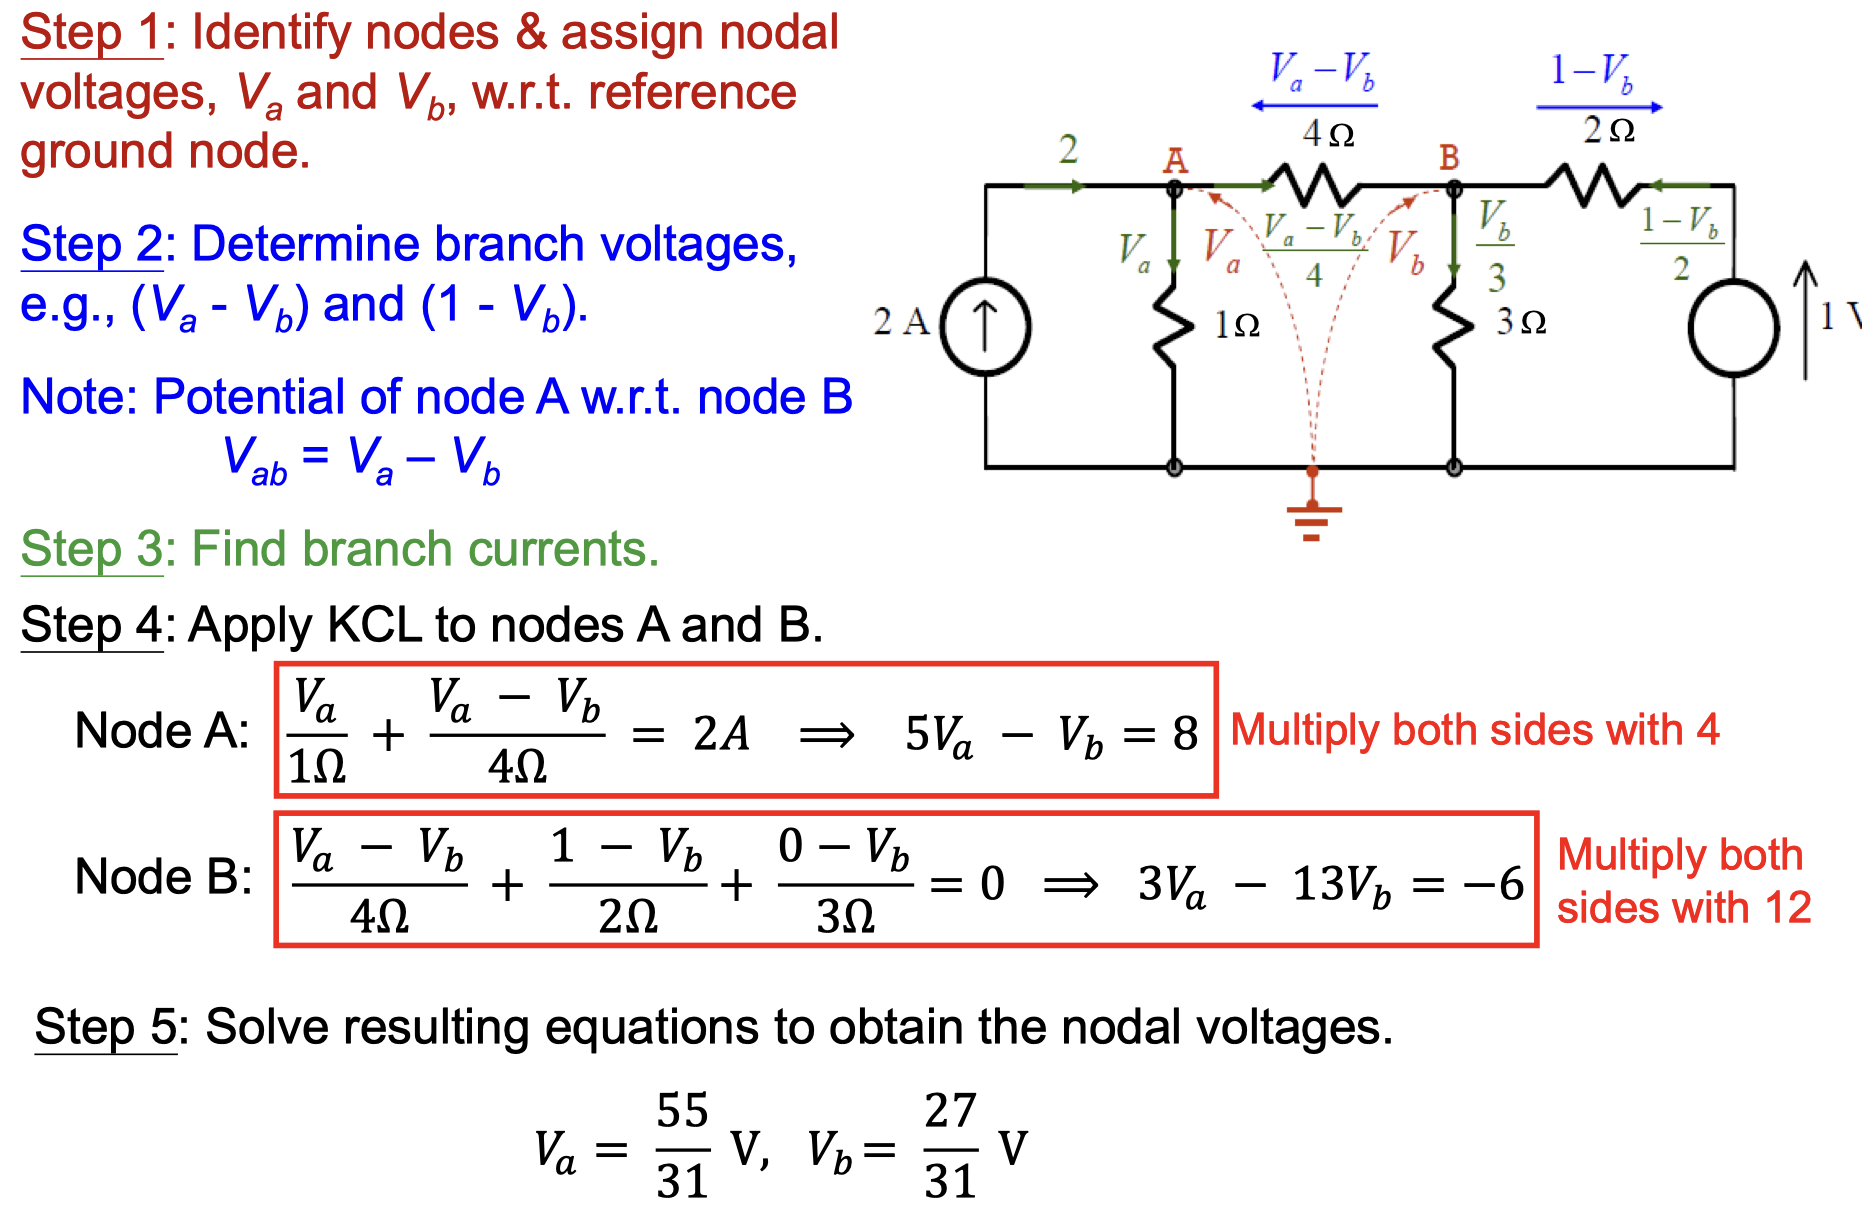
\includegraphics[width=0.75\linewidth]{image/KCL.png}
    \end{figure}
    \end{exam}
    \item Mesh Analysis KVL \\
    The sum of potential differences around any closed-loop is zero.
    \begin{center}
    \begin{circuitikz}[american]
        \draw (0,0) node[ground]{} to [battery2, invert, v=$V_A$] (0,2) -- (0,3)to  [R , R = $R_1$, v=$V_{R1}$] (3,3) to (3,3) to [R, R=$R_2$, v=$V_R2$](3,1) to [isource, l=$I_B$, v=$V_{IB}$](3,0) to node[ground]{} (3,0);
        \draw (3,3) to (5,3) to [R, R=$R_3$, v=$V_R3$](5,1) -- (5,0) to node[ground]{} (5,0);
    \end{circuitikz}
    \end{center}
    Loop 1: $V_A + (-V_{R1})+(-V_(R2))+(-V_{IB}) = 0$ \\
    Loop 2: $V_{IB}+V_{R2}+(-V_{R3}) = 0$\\
    Loop 3: $V_A + (-V_{R1})+(-V_{R3}) = 0$
    \item Linear Superposition \\
    When determining the impact of an individual source, you need to kill all other voltage source by short-circuiting them, and all other current source by open-circuiting them.
    \begin{figure}[h]
        \centering
        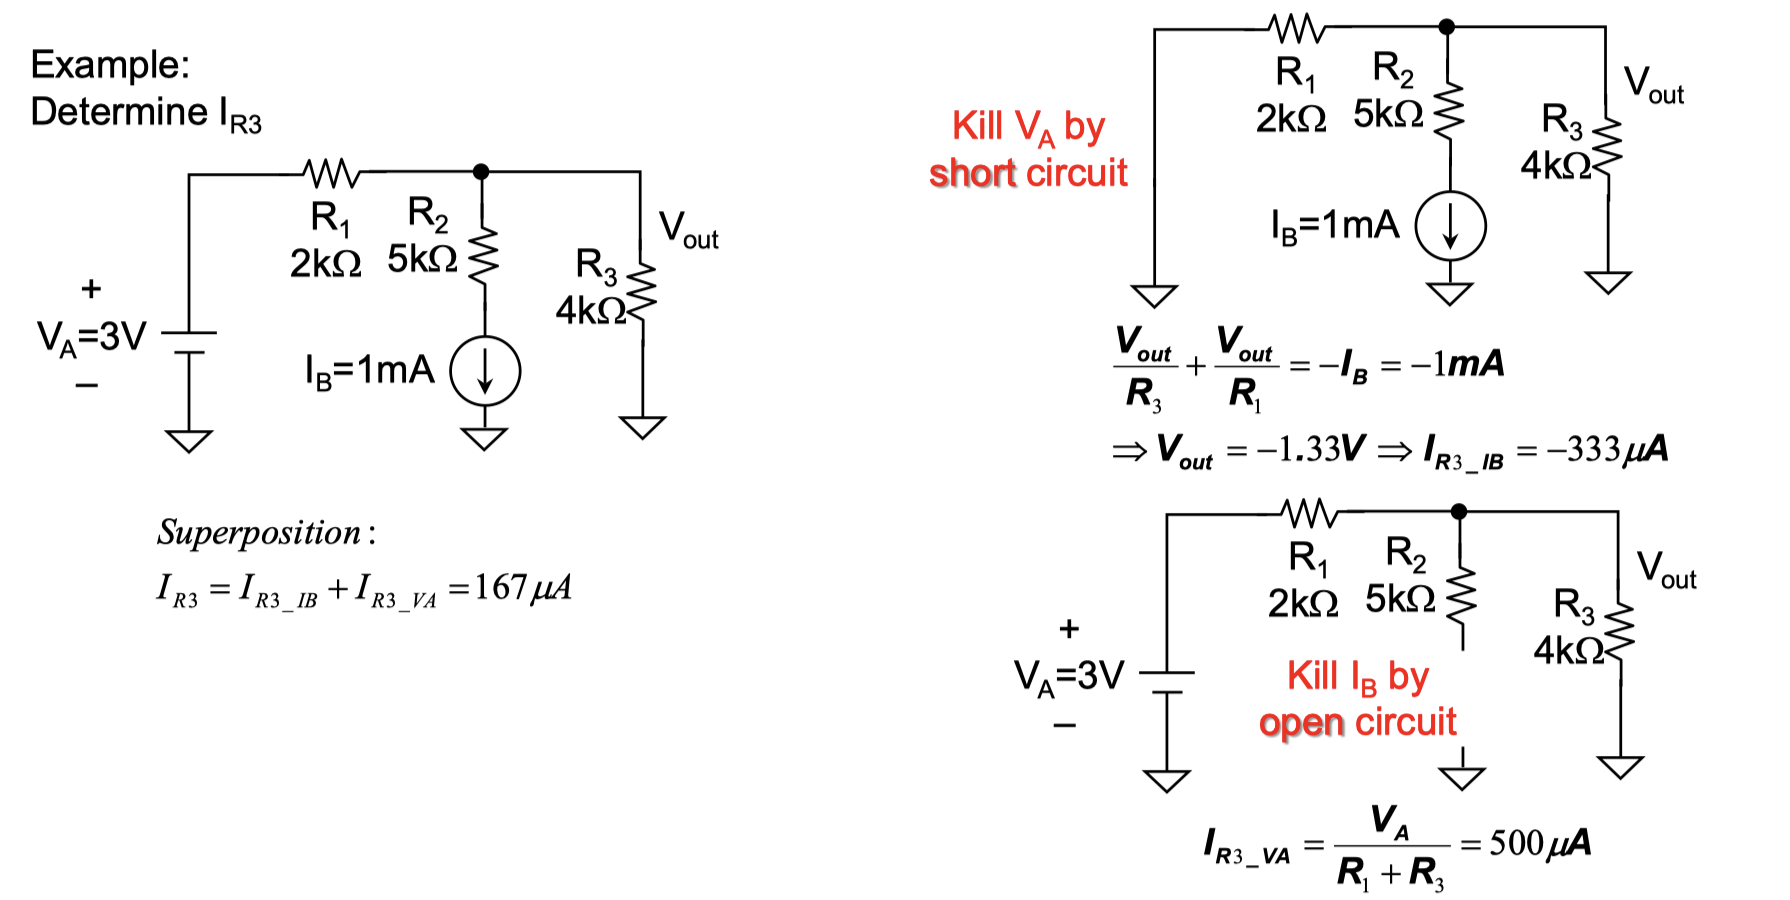
\includegraphics[width=0.8\linewidth]{image/linearsuper.png}
    \end{figure}
    \item Thevenin \& Norton Equivalent \\
    Thevenin Theorem: Any linear network with one port output can be replaced with an equivalent Thevenin voltage source $V_{THV}$ in series with a Thevenin resistance $R_{THV}$. \\
    Steps for Thevenin theorem :
    \begin{enumerate}
        \item Replace the port as an open circuit.
        \item Replace independent voltage source with short-circuit.
        \item Replace independent current source with open circuit.
        \item Calculate the $R_{THV}$ of the circuit.
        \item Calculate the $V_{THV}$ at the open port
        \item Re-draw the circuit with $V_{THV}$, $R_{THV}$ and $R$ at the open port to calculate $i$.
        \item $i$ will be the current flowing through your open port.
    \end{enumerate}
    Norton Theorem: \\
    Any linear network with one port output can be replaced with an equivalent Norton current source $I_{NOR}$ in parallel with a Norton resistance $R_{NOR}$.
    Steps for Norton theorem:
    \begin{enumerate}
        \item Replace the port as an open circuit.
        \item Replace independent voltage source with short-circuit.
        \item Replace independent current source with open circuit.
        \item Calculate the $R_{NOR}$ of the circuit.
        \item Calculate the $V_{THV}$ at the open port
        \item Calculate the $I_{NOR} = \frac{V_{THV}}{R_{NOR}}$.
        \item Re-draw the circuit with $I_{NOR}$, $R_{NOR}$ and $R_{load}$ as below to calculate $I_{load}$.
        \begin{center}
        \begin{circuitikz}[american]
            \draw (0,0) to [isource, l=$I_{NOR}$](0,3) to [short,-*](2,3) to [R,R=$R_{VOR}$](2,0) to (0,0);
            \draw (2,3) to [short, i=$I_{load}$](4,3) to [R, R=$R_{load}$](4,0) to [short,-*](2,0);
        \end{circuitikz}
        \end{center}
    \end{enumerate}
    \item AC Signal Quantities
    \begin{enumerate}
        \item Average value for AC signal
        \[v_{avg} = \frac{1}{T}\int^T_0v(t)dt\]
        \item Root-Mean-Square for AC
        \[v_{rms} = \sqrt{\frac{1}{T}\int^T_0v^2(t)dt}\]
    \end{enumerate}
    \item Phasor \\
    For AC Sinusoidal function \\
    Phasor $\underbrace{V = re^{j\theta} = r \angle \theta}_{\text{r is r.m.s}}$
    \item Capacitor
    \[i(t) = C\frac{dv(t)}{dt}\]
    Treat capacitor as open circuit in DC circuit analysis.\\
    Reactance of capacitor: $\displaystyle X_C = \frac{1}{j\omega C}$ \\
    Laplace Transformation: $\displaystyle V_C(s) = \frac{I(s)}{sC} \hspace{1cm} Z_C(s)=\frac{1}{sC}$ 
    \item Inductor
    \[v(t) = L\frac{di(t)}{dt}\]
    Treat inudctor as a short circuit in DC circuit analysis.\\
    Reactance of inductor: $\displaystyle X_L = j\omega L$ \\
    Laplace Transformation: $V_L(s)=sLI(s) \hspace{1cm} Z_L(s)=sL$
    \item Impedance and Admittance\\
    Impedance: Resistance + Reactance
    \[Z = R + jX\]
    Admittance: Conductance + Susceptance
    \begin{align*}
        Y &= \frac{1}{Z} = G +j B \\
        G &= \frac{R}{R^2 + X^2} \\
        B &= \frac{-X}{R^2 + X^2}\\
    \end{align*}
    \item RC Circuits \\
    Passive $1^{st}$ Order Low Pass Filter
        \begin{center}
            \begin{circuitikz}
                \draw
                (0,0)
                to[R, l=$R_1$, o-] (3,0)
                -- (3,-0.5)
                to[C, l=$C_1$] (3,-2)
                node[ground]{}
                (3,0)
                to[short, -o] (4,0)
                node[right] {$V_{\text{out}}$}
                (0,0)
                node[left] {$V_{\text{in}}$};
            \end{circuitikz}
        \end{center}
        $\displaystyle H(j\omega) = \frac{V_{\text{out}}}{V_{\text{in}}} = \frac{\frac{1}{j\omega C_1}}{\frac{1}{j\omega C_1} + R_1} = \frac{1}{j\omega C_1 R_1 + 1}$\\
        $3dB$ Gain \\
        \begin{enumerate}
            \item Since $\displaystyle |H(j\omega_{3dB})| = \frac{1}{\sqrt{2}}$ \\
            \item $\displaystyle \frac{1}{\sqrt{(\omega_{3dB}R_1C_1)^2+1}} = \frac{1}{\sqrt{2}}$  \\
            \item $\displaystyle \omega_{3dB} = \frac{1}{R_1C_1} $ \\
            \item $\displaystyle f_{3dB} = \frac{1}{2\pi R_1C_1}$
        \end{enumerate}
        \pagebreak
        Passive $1^{st}$ Order High Pass Filter
        \begin{center}
            \begin{circuitikz}
                \draw
                (0,0)
                to[C, l=$C_1$, o-] (3,0)
                -- (3,-0.5)
                to[R, l=$R_1$] (3,-2)
                node[ground]{}
                (3,0)
                to[short, -o] (4,0)
                node[right] {$V_{\text{out}}$}
                (0,0)
                node[left] {$V_{\text{in}}$};
            \end{circuitikz}
        \end{center}
        $\displaystyle H(j\omega) = \frac{V_{\text{out}}}{V_{\text{in}}} = \frac{R_1}{\frac{1}{j\omega C_1} + R_1} 
        = \frac{j\omega C_1 R_1}{j\omega C_1 R_1 + 1} = \frac{j\omega}{j\omega + \frac{1}{C_1 R_1}}$\\
        $3dB$ Gain\\
        Same logic as above, $\displaystyle f_{3dB} = \frac{1}{2\pi R_1C_1}$
        \item Maximum Power Transfer
        \begin{figure}[h]
            \centering
            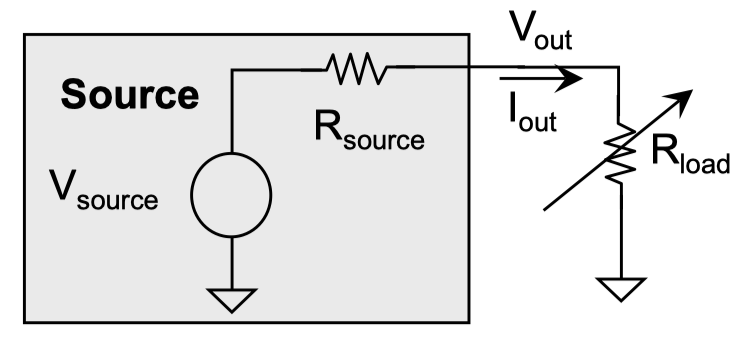
\includegraphics[width=0.75\linewidth]{image/powersource.png}
        \end{figure}
        \begin{align*}
        P_{\text{out}} &= \frac{V_{\text{source}}}{R_{\text{source}} + R_{\text{load}}} \times \frac{R_{\text{load}} V_{\text{source}}}{R_{\text{source}} + R_{\text{load}}} \\
        &= \frac{R_{\text{load}} V_{\text{source}}^2}{(R_{\text{source}} + R_{\text{load}})^2} \\
        \frac{dP_{\text{out}}}{dR_{\text{load}}} &= \frac{1}{(R_{\text{source}} + R_{\text{load}})^2} - \frac{2R_{\text{load}}}{(R_{\text{source}} + R_{\text{load}})^3} = 0 \\
        \Rightarrow R_{\text{load}} &= R_{\text{source}}
        \end{align*}
        Therefore, We can conclude that the maximum power transfer occurs when the $R_{\text{load}} = R_{\text{source}}$.
        \item Transients RC Circuits\\
        The transient state of a circuits is right after the circuit being switched on or off before reaching the steady state.
        \begin{exam}
            Here is a typical example.
            \begin{figure}[h]
                \centering
                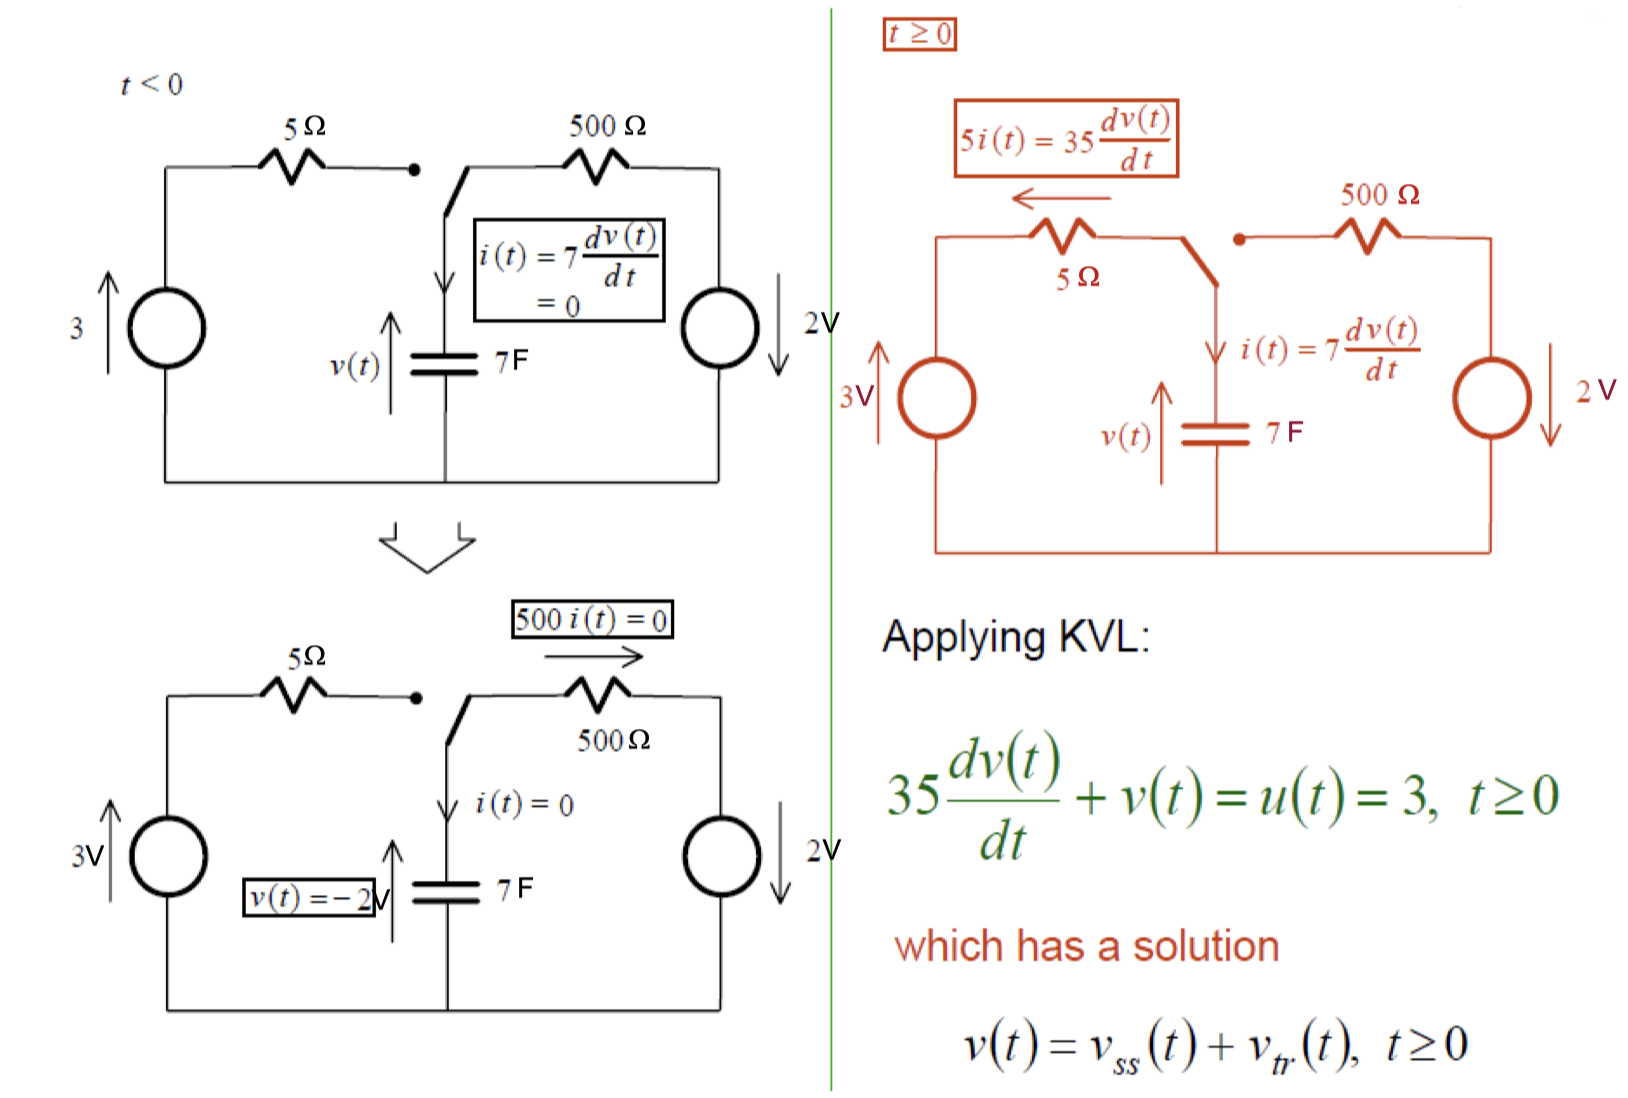
\includegraphics[width=0.75\linewidth]{image/transient.png}
            \end{figure}
        \end{exam}
        \item Power (instantaneous and average)
        \begin{figure}[h]
            \centering
            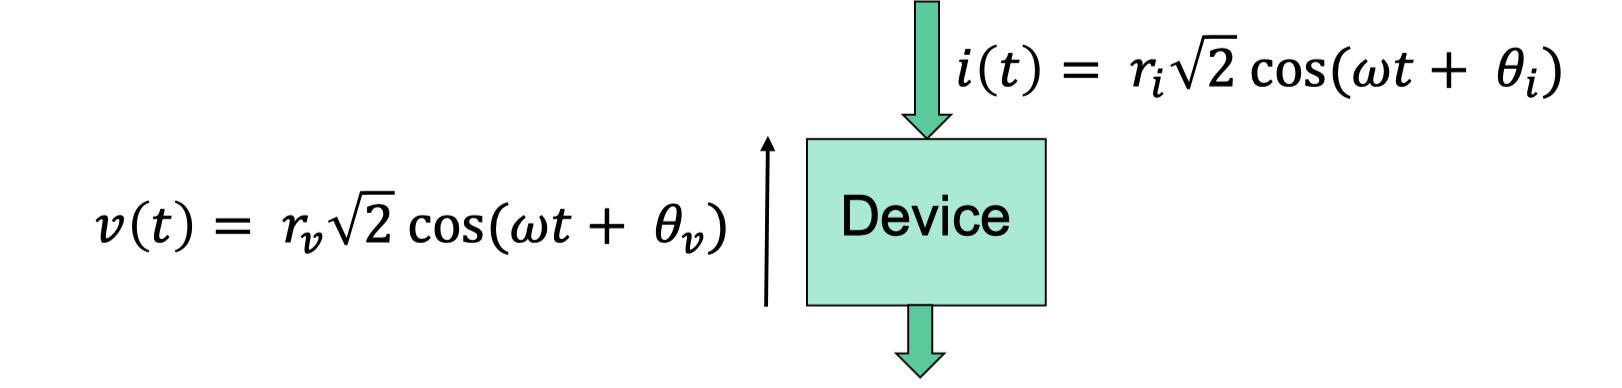
\includegraphics[width=0.75\linewidth]{image/poweri.png}
        \end{figure}\\
        For a given device, the instantaneous power can be derived in 
        \begin{align*} 
        p(t) & = i(t)v(t) \\
        &= 2r_ir_v \cos(\omega t + \theta_i) \cos(\omega t + \theta_v)\\ 
        &= r_ir_v(\cos(\theta_i - \theta_v) + \cos(2\omega t + \theta_i + \theta_v)) \\
        \end{align*} 
        Note the change from line 2 to line 3 is because $2 \cos(x_1) \cos(x_2) = \cos(x_1 - x_2) + \cos(x_1 + x_2)$
        \newpage
        The average power is 
        \begin{align*}
        P_{\text{av}} &= \frac{1}{T} \int_{0}^{T} p(t) dt \\
        &= \frac{r_i r_v}{T} \int_{0}^{T} \left[ \cos(\theta_i - \theta_v) + \cos\left(\frac{4\pi t}{T} + \theta_i + \theta_v\right) \right] dt \\
        &= r_i r_v \cos(\theta_i - \theta_v), \quad \text{where } T = \text{Period and } \omega = \frac{2\pi}{T} \\
        &= r_v r_i \cos(\theta_v - \theta_i) \\
        &= \Re\{r_v r_i e^{j(\theta_v - \theta_i)}\} \\
        &= \Re\{r_v r_i e^{j(\theta_i - \theta_v)}\} \\
        &= \Re\{V^* I\} \\
        &= \Re\{VI^*\} \\
        \end{align*}
        \item Power Factor
        \begin{enumerate}
            \item $\text{Real Power (Average)} = \Re[V^*I] = r_vr_i\cos(\theta_i-\theta_v)$
            \item  $\displaystyle \text{Apparent Power} = |V||I| = r_vr_i$
            \item Thus, $\displaystyle \text{Power Factor} = \frac{\text{Real Power}}{\text{Apparent Power}} = \cos(\theta_i-\theta_v)$ 
            \item When $V$ and $I$ are in phase, $\theta_i = \theta_v$ , power factor is unity.
            \item Leading Power Factor: $I$ leads $V$ where $\theta_i > \theta_v$ .
            \item Lagging Power Factor: $I$ lags $V$ where $\theta_i < \theta_v$.
        \end{enumerate}
\end{enumerate}
\subsubsection{Diode (pn-Junction)}
\begin{enumerate}
    \item Introduction
    \begin{enumerate}
        \item The diode to be discussed is a semiconductor pn-junction. Please see this \href{https://www.youtube.com/watch?v=Fwj_d3uO5g8}{link} before reading notes.
        \item p-type (\textbf{Holes}) impurity is a group \rom{3} elements (\ce{Br},\ce{Al},\ce{Ga})\\
        n-type (\textbf{Electrons}) impurity is a group \rom{5} elements (\ce{P},\ce{As},\ce{Sb})
        \item The process of doping can also change a p-type semiconductor to n-type semiconductor, and vice versa.
        \item Two types of charge carrier movement namely, drift and diffusion.
        \begin{enumerate}
            \item Drift current $I_{\text{Drift}}$ : Charge carriers move in the presence of electric field.
            \item Diffusion Current $I_{\text{Diffusion}}$ : Charge carriers diffuse owing to the difference in carrier concentration.
        \end{enumerate}
        \item IV Characteristic\\
            \begin{minipage}{0.4\textwidth}
            It allows current flow through it easily in one direction (forward direction), but not opposite directions (reverse direction), except for the reverse breakdown region.
            \end{minipage}
            \begin{minipage}{0.6\textwidth}
                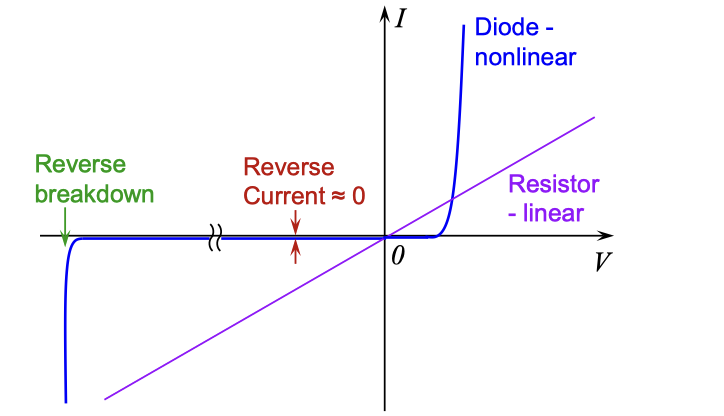
\includegraphics[width=1\linewidth]{image/pnchar.png}
            \end{minipage}
    \end{enumerate}
    \item Forward-Bias \\
    \begin{minipage}{0.4\textwidth}
        Under forward-bias, the p-type terminal is at a higher voltage with respect to the n-type terminal. \\
        The forward current remains small $\approx 0$ until the cut-in voltage and increases quickly with a small increase in $V$. \\
        The voltage drop across the diode lies in a narrow range.
    \end{minipage}
    \begin{minipage}{0.6\textwidth}
        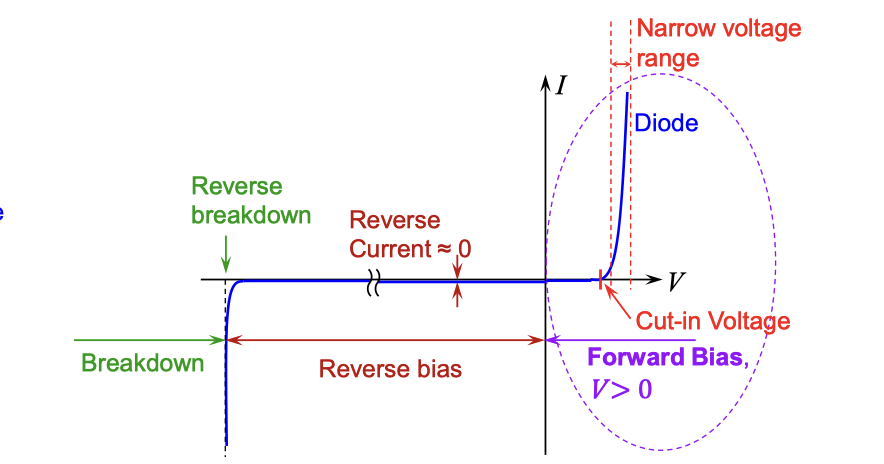
\includegraphics[width=1\linewidth]{image/diodeforawd.png}
    \end{minipage}
    \item Reverse-Bias \\
    \\
    \begin{minipage}{0.4\textwidth}
        Under reverse-bias $V<0$, an external voltage is applied such that the p-type terminal is at a lower voltage with respective to the n-type terminal. \\       
        For $\displaystyle |V| = V_R < V_Z$, the breakdown voltage reverse current is very small and can be treated as 0.
    \end{minipage}
    \begin{minipage}{0.6\textwidth}
        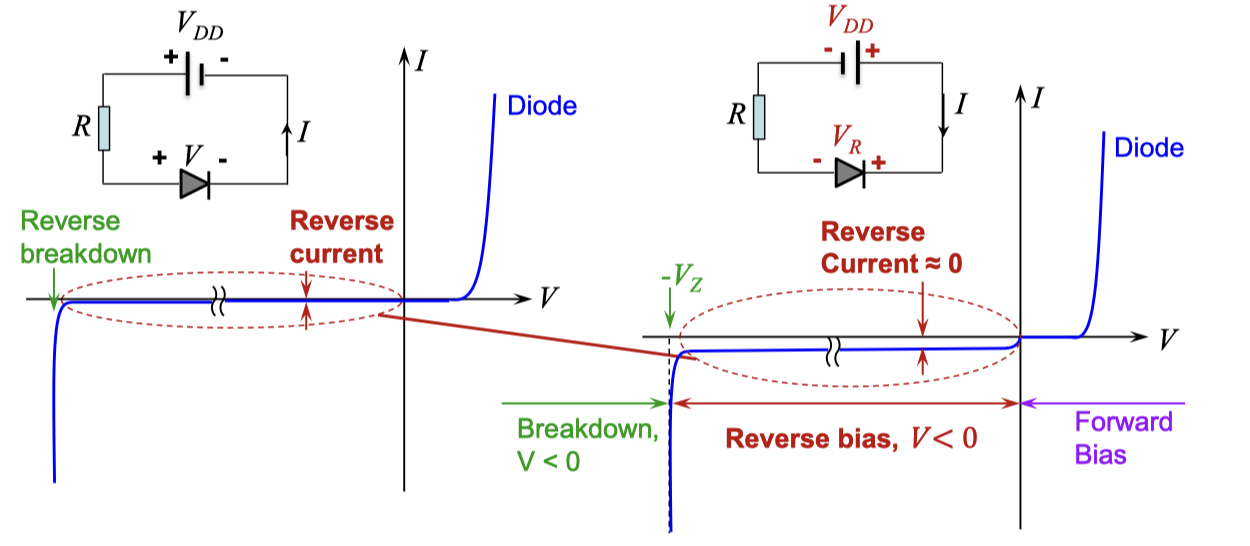
\includegraphics[width=1\linewidth]{image/reversebias.png}
    \end{minipage}
    \item Breakdown Region\\
    \\
    \begin{minipage}{0.4\textwidth}
        When $\displaystyle V_{DD} > V_Z$, the current can be very large, while its voltage is practically not changed and stays at $-V_Z$. This is called \textbf{Breakdown}\\
        The current can be limited by connecting a resistor $R$ in series with the pn junction diode. $\displaystyle I = \frac{V_{DD}-V_Z}{R}$
    \end{minipage}
    \begin{minipage}{0.6\textwidth}
        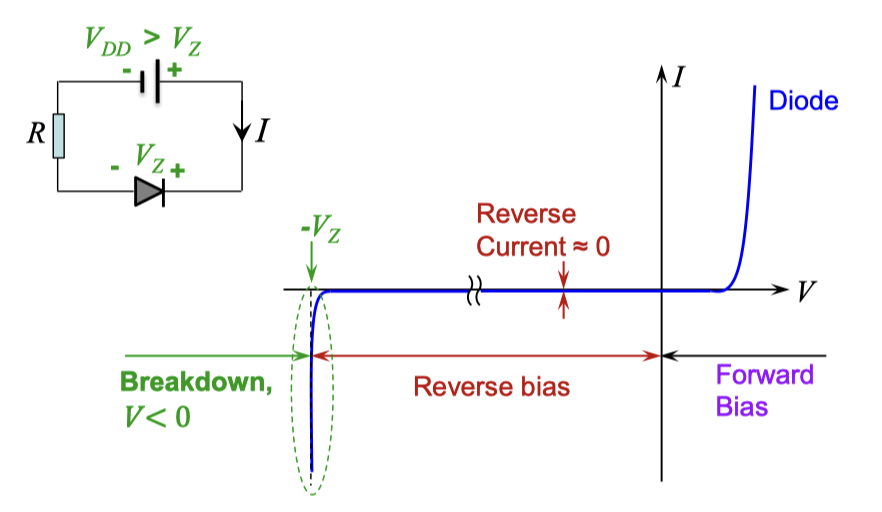
\includegraphics[width=1\linewidth]{image/breakdownregion.png}
    \end{minipage}
    \item Current Voltage Characteristic
    \[I = I_S(e^{\frac{V}{nV_T}}-1)\]
    \begin{enumerate}
        \item $V$ is the voltage across the diode.
        \item  $I$ is the current flowing through the diode.
        \item $V_T$ is thermal voltage, $\displaystyle V_T = \frac{kT}{q} = 0.0259V \approx 0.025V \approx 0.026V$ at $T = 300K$.
        \item $n$ is exponential factor between 1 and 2, where $n = 1$ is for an ideal pn-junction diode.
        \item $I_S$ is reverse saturation current, increases with increasing temperature.
    \end{enumerate}
    In substantial \textbf{Forward-Bias} ($V>$ cut-in voltage $> 0$), and $\displaystyle e^{\frac{V}{nV_T}} >> 1$ and therefore
    \[I = I_S(e^{\frac{V}{nV_T}}-1) \approx I_S e^{\frac{V}{nV_T}}\quad \text{or} \quad V\approx nV_T\ln(\frac{I}{I_S})\]
    $I \approx 0$ for $V < ~0.5V$, this is the cut-in voltage.\\
    The voltage drop across diode is around $0.6V$ to $0.8V$, usually we take as $0.7V$.\\
    In \textbf{Reverse-Bias} $V<0$, for $|V|>$ a few times $nV_T$ and $\displaystyle e^{\frac{V}{nV_T}} << 1$ and therefore
    \[I = I_S(e^{\frac{V}{nV_T}}-1) \approx -I_S\]    
    \newpage
    \item Large Signal Model
    \begin{figure}[h]
        \centering
        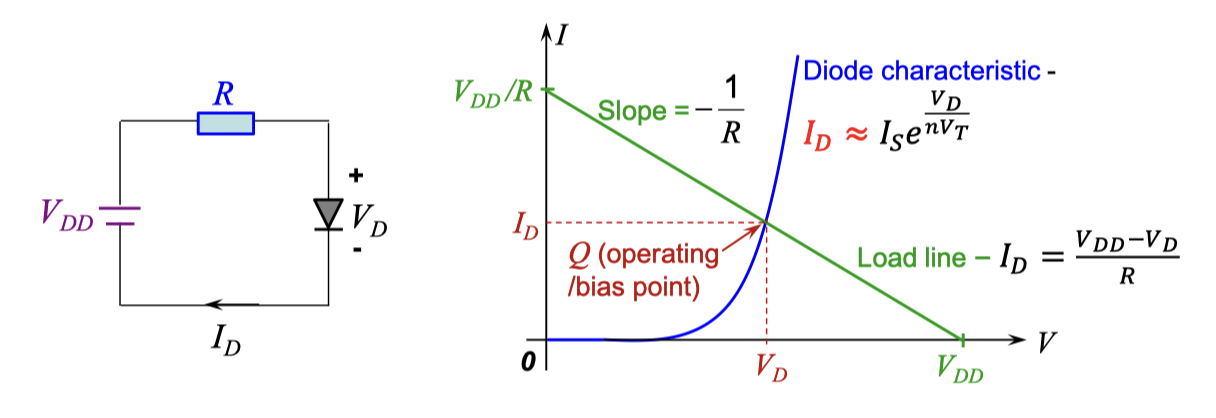
\includegraphics[width=1\linewidth]{image/largemodel.png}
    \end{figure} \\
    For a diode in forward-bias, assuming $\displaystyle V_{DD}>0.5V$ the IV characteristic is
    \[I_D \approx I_S e^{\frac{V_D}{nV_T}}\]
    $\displaystyle I_d \text{and} V_D$ are also governed by KVL where 
    \[I_D = \frac{V_{DD}-V_D}{R}\]
    Since, $I_D$ and $V_D$ cannot be determined easily by solving equations above. The can be solved graphically, or by iterative procedure. \\
    Here are the example of a circuit with \(nV_T = 0.043\) \\
    \begin{enumerate}
        \item We first assume \( V_D = V_{D0} = 0.7 \, \text{V} \).
        \item Next, substitute \( V_D = V_{D0} = 0.7 \, \text{V} \) into equation the KVL equation, we make an initially estimate for \(I_{D0} = \frac{V_{DD} - V_{D0}}{R} = \frac{5 - 0.7}{1000} = 4.3 \, \text{mA} \)
        \item Using the estimated \( I_{D0} = 4.3 \, \text{mA} \), a better estimate for \( V_D ( = V_{D1} ) \) is obtained using the diode equation
        \[ V_D - 0.6 \, \text{V} = nV_T \ln(\frac{I_D}{I_{1} mA}) \Rightarrow V_{D1} - 0.6 \, \text{V} = 0.043 \ln(\frac{4.3 \, \text{mA}}{1 \, \text{mA}}) \]
        \[ \Rightarrow V_{D1} = 0.6627 \, \text{V} \]
        \item Substitute \( V_{D1} = 0.6627 \, \text{V} \) into equation, a better estimate for \( I_D ( = I_{D1} ) \) is obtained
        \[ I_{D1} = \frac{V_{DD} - V_{D1}}{R} = \frac{5 - 0.6627}{1000} = 4.3373 \, \text{mA} \]
        \item Thus, after the 1st iteration \( I_{D1} = 4.3373 \, \text{mA} \) and \( V_{D1} = 0.6627 \, \text{V} \). The 2nd iteration proceeds in a similar manner, by repeating steps 3 and 4:
        \[ V_{D2} - 0.6 \, \text{V} = 0.043 \ln(\frac{4.3373 \, \text{mA}}{1 \, \text{mA}}) \Rightarrow V_{D2} = 0.6631 \, \text{V} \]
        \[ I_{D2} = \frac{V_{DD} - V_{D2}}{R} = \frac{5 - 0.6631}{1000} = 4.3369 \, \text{mA} \]
        \item 2nd iteration yields \( I_{D2} = 4.3369 \, \text{mA} \) and \( V_{D2} = 0.6631 \, \text{V} \), which are close to values obtained after the 1st iteration (less than 0.06\% difference), hence further iterations are not necessary, as the values of \( V_D \) and \( I_D \) have converged.
    \end{enumerate}
    As such, in order for easier calculation, we need to model diode.\\
    \begin{figure}[h]
        \centering
        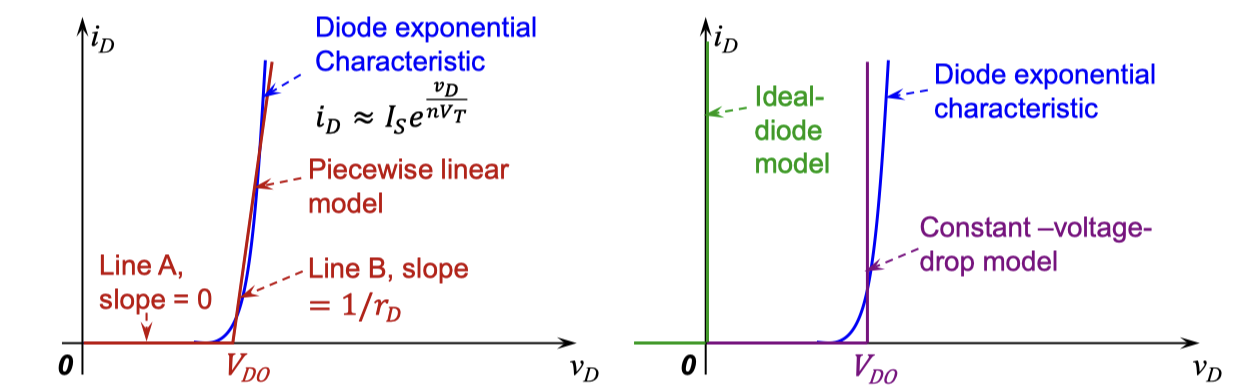
\includegraphics[width=1\linewidth]{image/largemodeling.png}
    \end{figure}
    \begin{enumerate}
        \item Piecewise-linear model: \(i_D = 0,\; \text{for}\; v_D\leq V_{D0}\) \\
        \(i_D = \frac{v_D - V_{D0}}{r_D}, \text{for} \; v_D \geq V_{D0}\)
        \item Ideal-diode model: \(V_{D0} = 0, \; r_D = 0\)
        \item Constant-voltage-drop model: \(r_D = 0, V_{D0} \; \text{is taken as} \; 0.7V.\) \\
        In constant-voltage-drop model, treat diode as a $0.7V$ drop and then calculate the rest.
    \end{enumerate}
    \newpage
    \item Small Signal Model \\
    This model are used with circuits with time varying signal (AC) in addition to the DC supply as shown in the graph below.
    \begin{figure}[h]
        \centering
        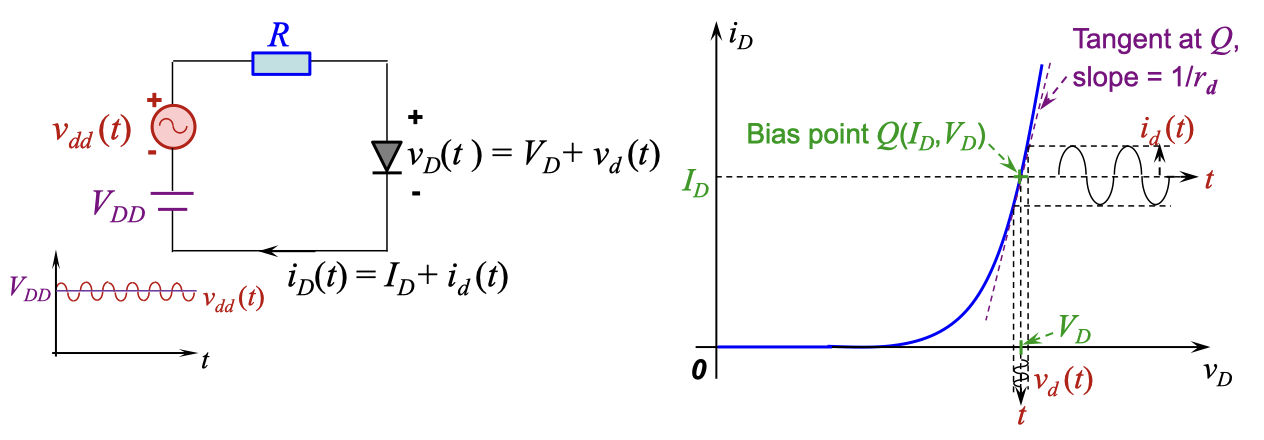
\includegraphics[width=1\linewidth]{image/smallsignalmodel.png}
    \end{figure}\\
    Calculation for such signal can be derived into two parts.
    \begin{enumerate}
        \item DC analysis, consider only $V_{DD}$, 
        \item AC analysis, consider only $v_{dd}(t)$
        \item Last, using superposition to give the total effect.
    \end{enumerate}
    Small-Signal Operation:
    \begin{enumerate}
        \item Find $I_D$ and $V_D$ using Large Signal Model.
        \item With a small signal source $v_{dd}(t)$
        \[i_D(t) = I_S e^{\frac{v_D(t)}{nV_T}} = I_S e^{\frac{V_D + v_d(t)}{nV_T}} = I_S e^{\frac{V_D}{nV_T}} e^{\frac{v_d(t)}{nV_T}} = I_D e^{\frac{v_d(t)}{nV_T}}\]
        \[\approx I_D[1+\frac{v_d(t)}{nV_T}] = I_D + \frac{I_D}{nV_T}v_d(t)\]
        Note, {\color{red}{\(e^x \approx 1 + x\)}} for $x < 1$ .
        \item Hence, $\displaystyle i_d(t) = \frac{I_D}{nV_T}v_d(t) = \frac{1}{r_d}v_d(t)$
        \item \(r_d = \frac{nV_T}{I_D}\), $r_d$ is called diode small-signal resistance.
        \item Since $r_d$ having a unit as $\Omega$, You can model the diode as a small resistor.
        \item \(i_d(t) = \frac{v_{dd}(t)}{R+r_d}\), Using KVL we can obtain the small-signal current.
        \item The slope at the DC bias point Q, givese the approximatelt the inverse of diode small-signal resistance $r_d$
        \[\frac{\partial i_D}{\partial v_D} \bigg|_{v_D = V_D} = \frac{1}{r_d} = \frac{i_d}{v_d} = \frac{I_D}{nV_T}\]
        \item $r_d$ is also known as the diode incremental resistance.
    \end{enumerate}
    \item Rectifier and Voltage Regulator\\
    Half-way Rectifier\\
    \begin{figure}[h]
        \centering
        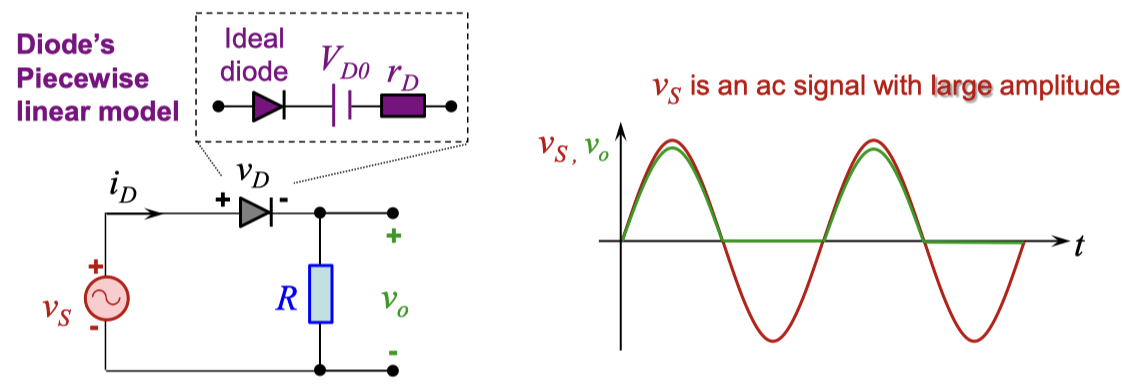
\includegraphics[width=1\linewidth]{image/halfrect.png}
    \end{figure} \\
    In the positive half, \(v_o = v_S -V_{D0}\) \\
    In the negative half, \(v_o = 0\) \\
    Full-wave Bridge rectifier\\
    \begin{figure}[h]
        \centering
        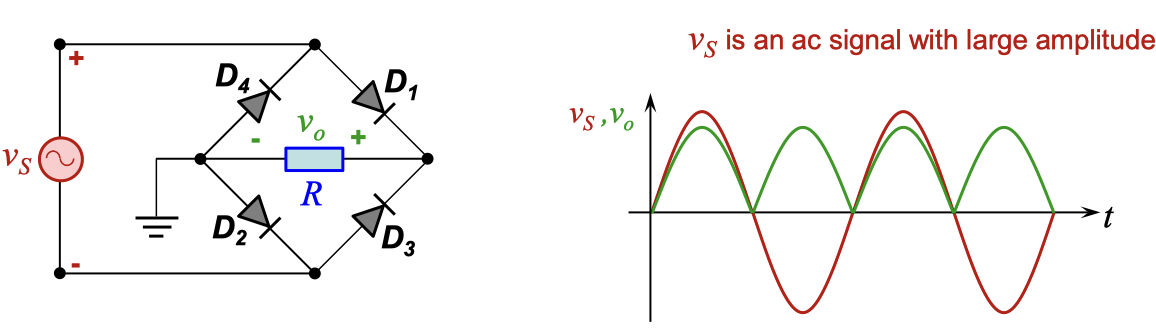
\includegraphics[width=1\linewidth]{image/fullwavebridge.png}
    \end{figure} \\
    Since there are two diodes involved, \(v_o = V_S - 2\times V_{D0}\) 
    \newpage
    Zener diode as voltage reference
    \begin{figure}[h]
        \centering
        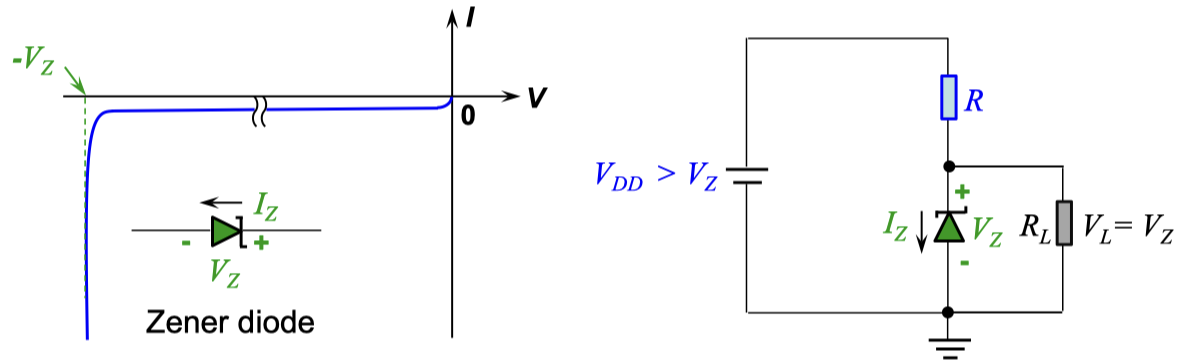
\includegraphics[width=1\linewidth]{image/zener.png}
    \end{figure}\\
    Since $V_Z$ is operating in the breakdown region, $R_L$'s voltage can be regulated by $V_Z$ as $V_L=V_Z$. Note that $I_Z \neq 0$.
    \item Charge stored and capacitance effect
    \begin{figure}[h]
        \centering
        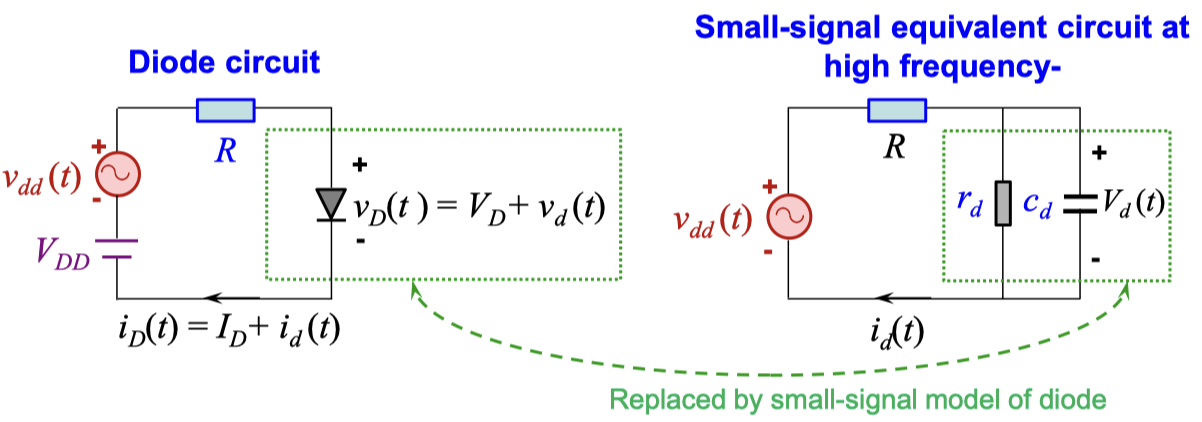
\includegraphics[width=1\linewidth]{image/diodesmall-signal.png}
    \end{figure}
\end{enumerate}
\subsubsection{Operational Amplifier}
\begin{enumerate}
    \item Opamp Schematic
    \begin{figure}[h]
        \centering
        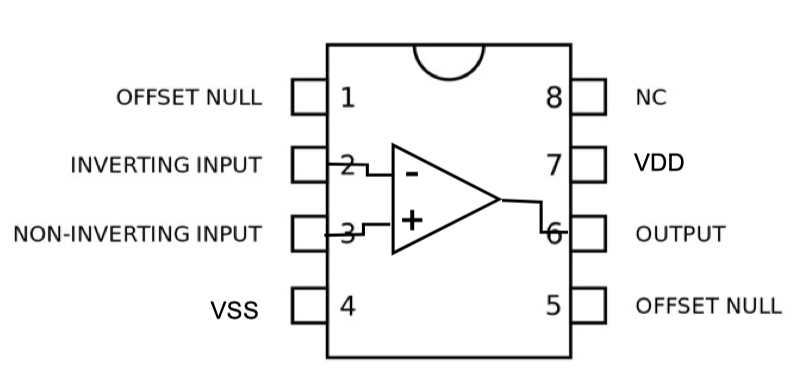
\includegraphics[width=0.5\linewidth]{image/opamp.png}
    \end{figure} \\
    For an ideal Opamp, $A = 10000 \rightarrow \infty$
    \item Inverting Amplifier\\
    \begin{circuitikz}
        \draw
        (0,0) node[op amp] (opamp) {}
        (opamp.+) node[left] {}
        (opamp.-) node[left] {}
        (opamp.out) node[right] {}
        (opamp.up) -- ++(0,0.5) node[vcc]{\(V_{CC}\)}
        (opamp.down) -- ++(0,-0.5) node[vee]{\(V_{EE}\)}
        
        % Inverting input
        (opamp.-) -- ++(-1.5,0) to[R, l_=\(R_{1}\), o-] ++(-2,0) node[left] {\(V_{in}\)}
        % Feedback resistor
        (opamp.-) ++(-1.5,0) -- ++(0,1.5) to[R, l=\(R_2\)] ++(3,0) -| (opamp.out)
        % Output
        (opamp.out) -- ++(1,0) node[right] {\(V_{out}\)}
        % Ground
        (opamp.+) -- ++(0,-0.5) node[ground] {};
    \end{circuitikz} \\
    The transfer function for inverting Amplifier is 
    \begin{equation}
        \frac{v_{out}}{v_{in}} = -\frac{R_2}{R_1}
    \end{equation}
    Proof: \\
    \(v_1 = v_{\_} \approx v_{+} = 0\) [Virtually short to ground] \\
    \(\displaystyle \frac{v_{in}-v_1}{R_1} = \frac{v_1 - v_{out}}{R_2}\)\\
    \(\displaystyle \frac{v_{in}}{R_1} = \frac{-v_{out}}{R_2}\) \\
    \(\displaystyle \frac{v_{out}}{v_{in}} = -\frac{R_2}{R_1}\)
    \item Non-Inverting Amplifier
    \begin{center}
        \begin{figure}[h]
            \centering
            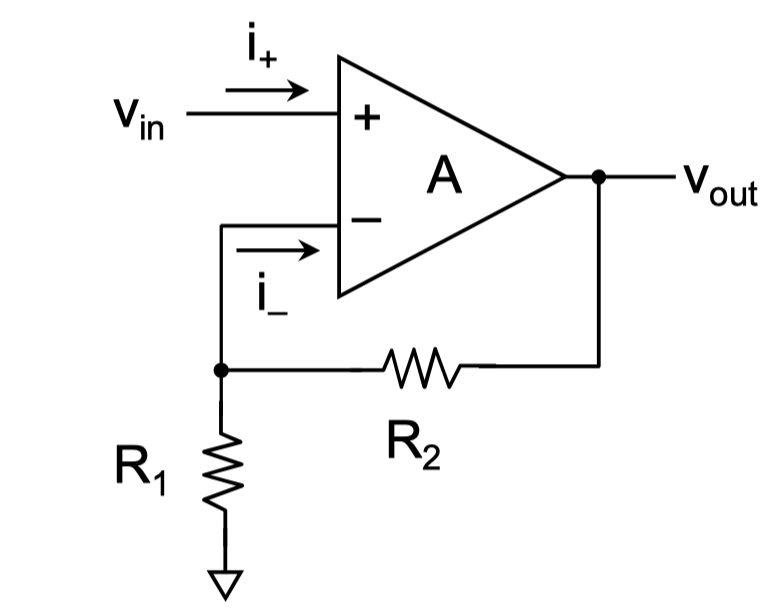
\includegraphics[width=0.4\linewidth]{image/noninopamp.png}
        \end{figure}
    \end{center}
    The transfer function for Non-Inverting Amplifier is 
    \begin{equation}
        \frac{v_{out}}{v_{in}} = (1+\frac{R_2}{R_1})
    \end{equation}
    Proof: \\
    $\displaystyle v_{\_} \approx v_{+} = v_{in}$ [Virtually short to ground] \\
    $\displaystyle v_{\_} = v_{out} \times \frac{R_1}{R_1 + R_2} = v_{in}$ [$i_{+} = i_{\_} = 0$]
    $\displaystyle \frac{v_{out}}{v_{in}} = (1+\frac{R_2}{R_1})$
    \item Unity Gain Buffer (Source follower) 
    %image here \\
    \begin{equation}
        \frac{v_{out}}{v_{in}} = 1
    \end{equation}
    \item Opamp Parameters ($A_{OL}$ and CMRR) \\
    The ratio of differential voltage amplification to common-mode voltage amplification.
    \begin{equation}
        \text{CMRR} = 20\log(\frac{A_{OL}}{A_{CM}}) = 20\log(A_{OL})-20\log(A_{CM})
    \end{equation}
    \item Opamp Parameters (Gain-BandWdith product) 
    \begin{equation}
        \text{GBW} = A_{OL} \times f_{3dB}
    \end{equation}
    For a inverting amplifier the $\omega_{3dB} = 2\pi \times \text{GBW} \times \frac{R_1}{R_1+R_2}$
    \item Opamp Parameters (Input Noise $V_n$) 
    \begin{equation}
        v_{noise,rms} = \sqrt{V_n^2\times f_{3dB}\times\frac{\pi}{2}}
    \end{equation}
    \item Opamp Parameters (PSRR) \\
    PSRR is a measure of how good the opamp rejects the supply line ripples or interference ($v_i,sup$).
    \begin{equation}
        \text{PSRR} = \frac{A_{OL}}{A_{SUP}}
    \end{equation}
    \item Opamp Parameters (Slew Rate) 
    \begin{equation}
        \frac{dv_{out}}{dt} = 2\pi f \times v_{out,peak}\sin{2\pi ft} < \text{SR}
    \end{equation}
    \item Summing Amplifier \\
    \begin{minipage}{0.5\textwidth}
        \begin{equation}
        V_{out} = -(v_1+v_2+v_3) \text{if $R_1=R_2=R_3=R$}
    \end{equation}
    \end{minipage}
    \begin{minipage}{0.5\textwidth}
        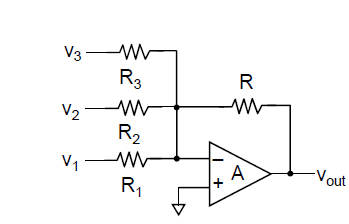
\includegraphics[width=0.75\linewidth]{image/summingamp.png}
    \end{minipage}
    \item Logarithmic Amplifier \\
    \begin{minipage}{0.5\textwidth}
        \begin{equation}
        V_{out} = -V_T\ln{\frac{I_in}{I_S}}
    \end{equation}
    \end{minipage}
    \begin{minipage}{0.5\textwidth}
        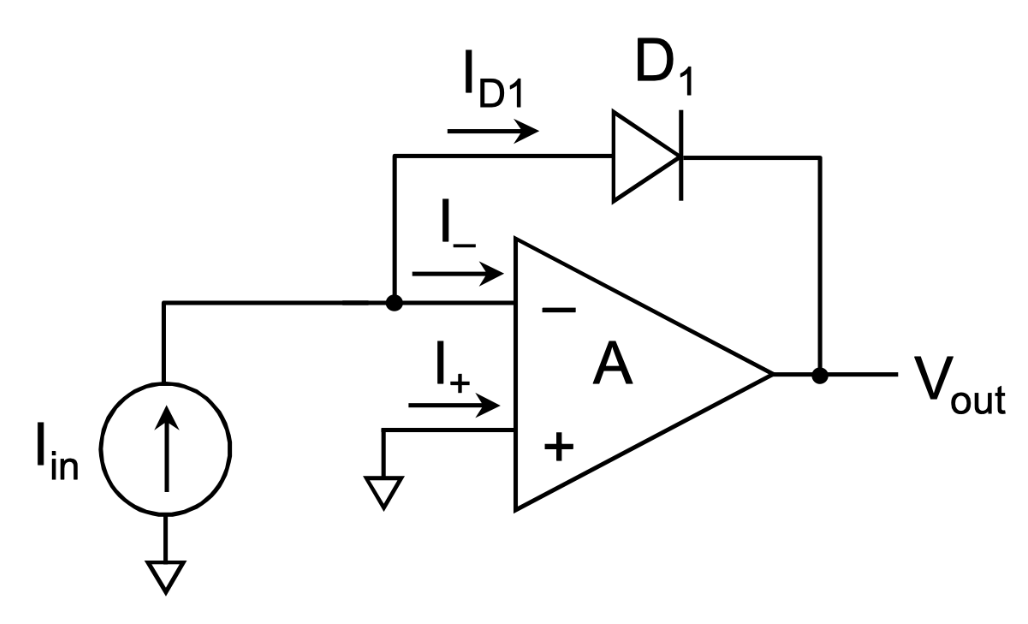
\includegraphics[width=0.7\linewidth]{image/logamp.png}
    \end{minipage}
    \item Exponential Amplifier \\
    \begin{minipage}{0.5\textwidth}
        \begin{equation}
        V_{OUT} = -R_1I_Se^{\frac{V_{IN}}{V_T}}
    \end{equation}
    \end{minipage}
    \begin{minipage}{0.5\textwidth}
        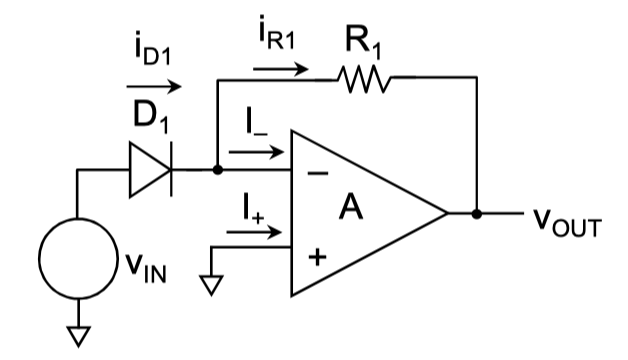
\includegraphics[width=0.7\linewidth]{image/expamp.png}
    \end{minipage}
    \item Instrumentation Amplifier \\
    \begin{minipage}{0.5\textwidth}
        \begin{equation}
            v_{out} = -\frac{R_2}{R_1}v_{id}
        \end{equation}
    \end{minipage}
    \begin{minipage}{0.5\textwidth}
            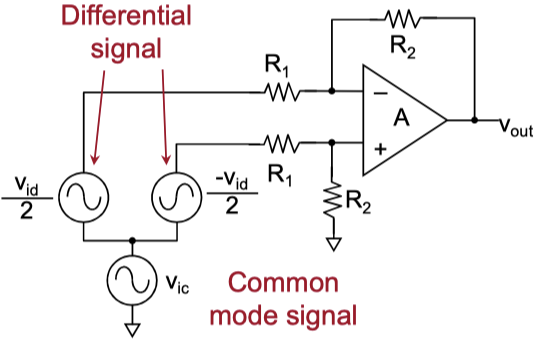
\includegraphics[width=0.75\linewidth]{image/instrumenamp.png}
    \end{minipage}
    \item Integrator \\
    \begin{minipage}{0.5\textwidth}
        \begin{equation}
            v_{out}(t)=-\frac{1}{RC}\int^t_0 v_{in}(t)dt
        \end{equation}
    \end{minipage}
    \begin{minipage}{0.5\textwidth}
        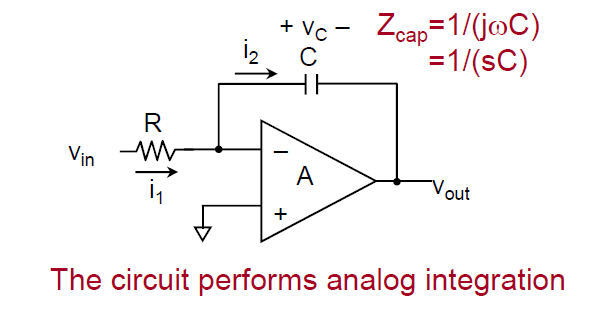
\includegraphics[width=0.75\linewidth]{image/integrator.png}
    \end{minipage}
    \item Differentiator \\
    \begin{minipage}{0.5\textwidth}
        \begin{equation}
            v_{out}(t)=-RC\frac{dv_{in}(t)}{dt}
        \end{equation}
    \end{minipage}
    \begin{minipage}{0.5\textwidth}
        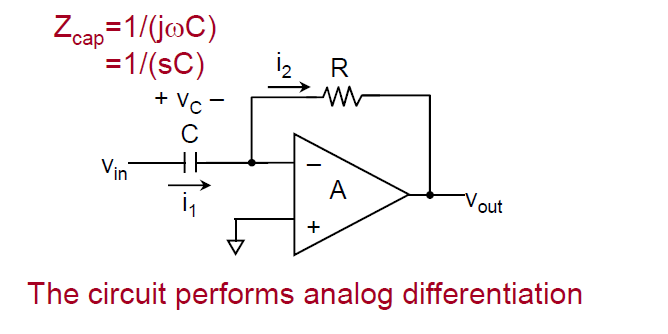
\includegraphics[width=0.75\linewidth]{image/differentiator.png}
    \end{minipage}
    \newpage
    \item Passive $1^{st}$ Order Lowpass Filter \\
    \begin{minipage}{0.5\textwidth}
        \begin{equation}
            \omega_{3dB}=\frac{1}{R_1C_1}
        \end{equation}
    \end{minipage}
    \begin{minipage}{0.5\textwidth}
        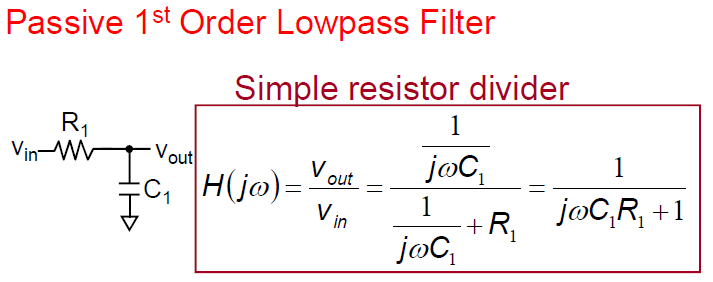
\includegraphics[width=0.75\linewidth]{image/1storderpassive.png}
    \end{minipage}
    \item Passive $1^{st}$ Order Highpass Filter \\
    \begin{minipage}{0.5\textwidth}
        \begin{equation}
            \omega_{3dB}=\frac{1}{R_1C_1}
        \end{equation}        
    \end{minipage}
    \begin{minipage}{0.5\textwidth}
        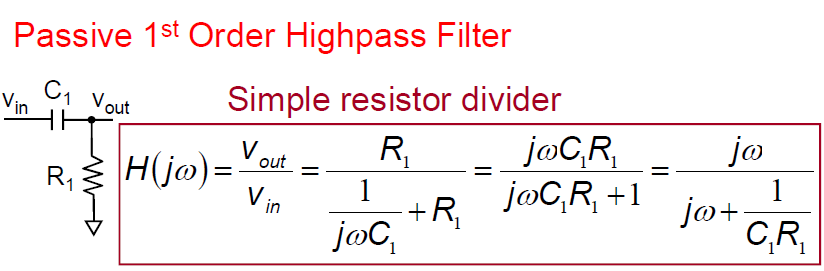
\includegraphics[width=0.75\linewidth]{image/1storderhigh.png}
    \end{minipage}
    \item Active $1^{st}$ Order Lowpass Filter
    \begin{figure}[h]
        \centering
        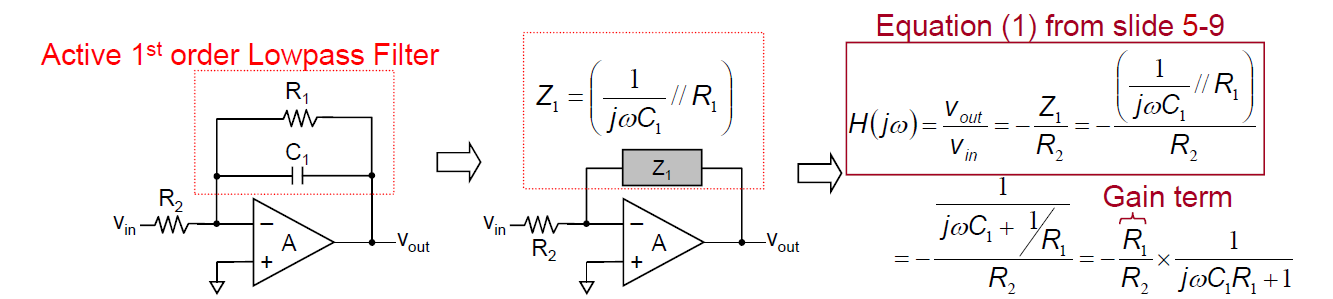
\includegraphics[width=0.75\linewidth]{image/1sactivelowe.png}
    \end{figure}
    \item Active $1^{st}$ Order Highpass Filter
    \begin{figure}[h]
        \centering
        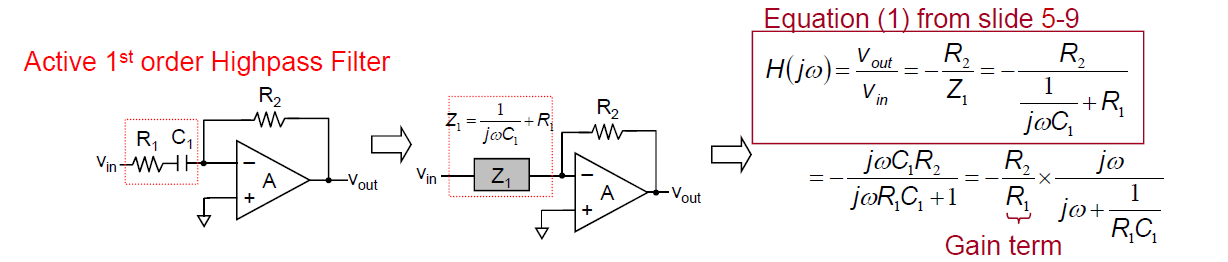
\includegraphics[width=0.78\linewidth]{image/1stactivehigh.png}
    \end{figure}
    \item \textit{Sallen-Key} Lowpass Filter 
    \begin{figure}[h]
        \centering
        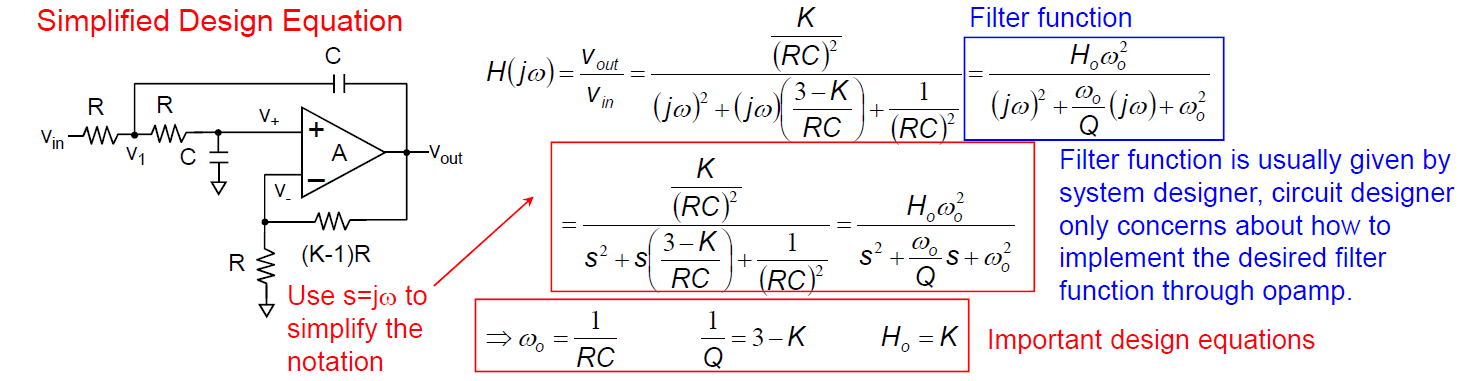
\includegraphics[width=0.75\linewidth]{image/ssklowpass.png}
    \end{figure}
    \newpage
    \item \textit{Sallen-Key} High Filter
    \begin{figure}[!h]
        \centering
        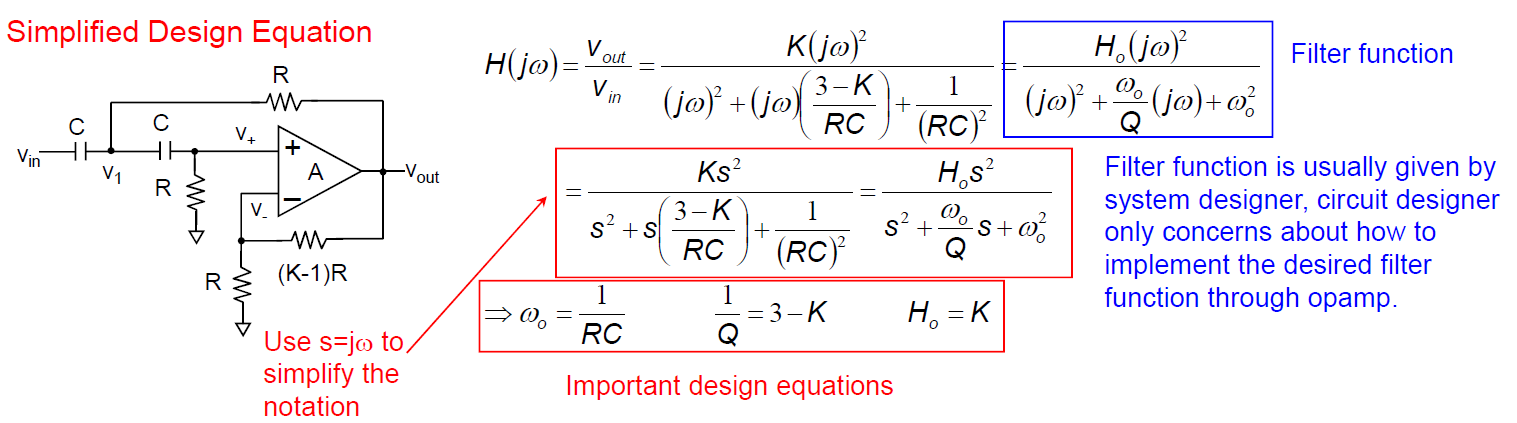
\includegraphics[width=0.75\linewidth]{image/skhighpass.png}
    \end{figure}
    \item Superdiode
    \begin{figure}[!h]
        \centering
        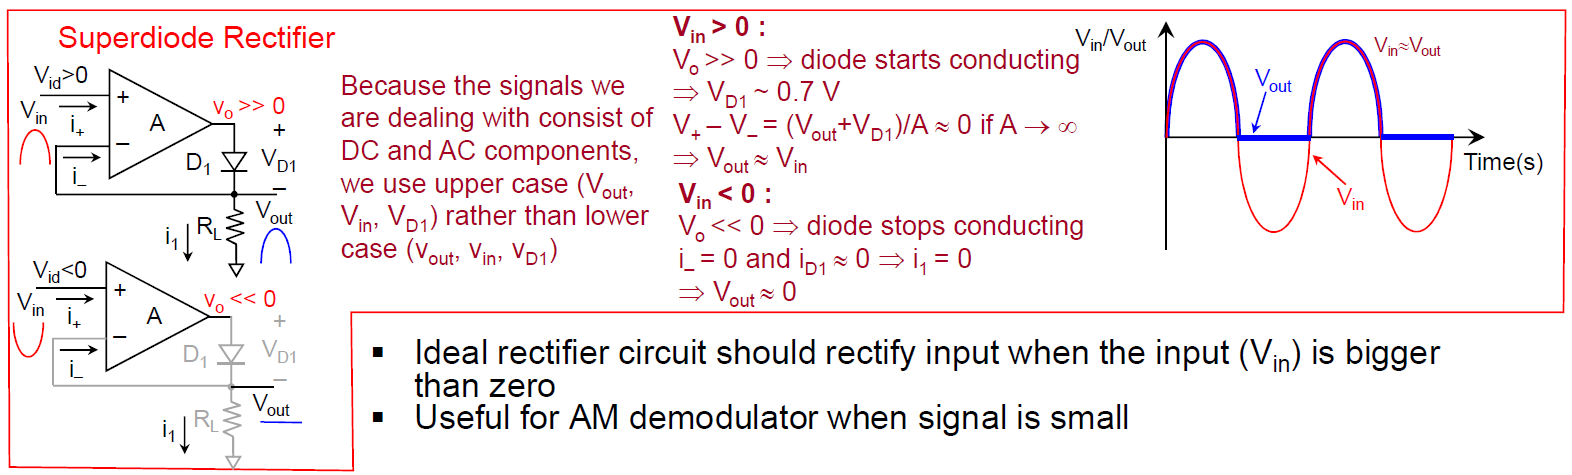
\includegraphics[width=0.75\linewidth]{image/superdiode.png}
    \end{figure}
    \item Comparator
    \begin{figure}[!h]
        \centering
        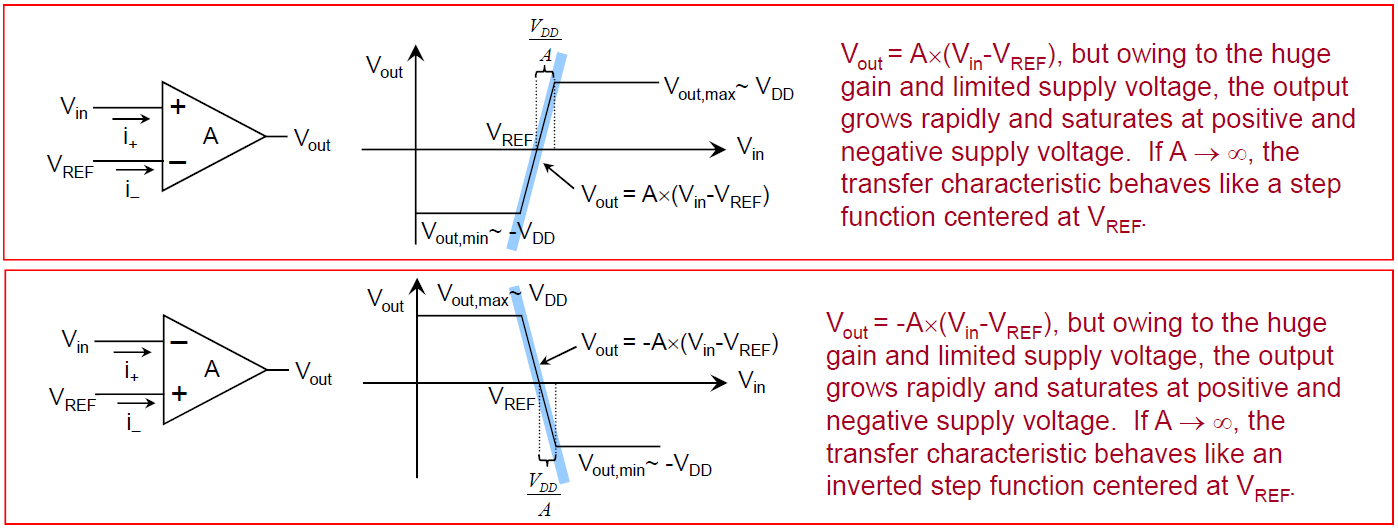
\includegraphics[width=0.75\linewidth]{image/comparator.png}
    \end{figure}    
\end{enumerate}

\newpage 
\subsubsection{Bipolar Junction Transistor}
\textbf{BJT} is a 3-terminal device made using a single crystal semiconductor (typically silicon), just like the pn-junction diode. \\
\textbf{Mode of NPN BJT}
\begin{table}[ht]
\centering
\caption{Transistor Modes of Operation.}
\label{table:transistor_modes}
\small % Or \footnotesize or \scriptsize
\begin{tabularx}{\textwidth}{|X|X|X|X|}
\hline
\textbf{Mode of Operation} & \textbf{Emitter-Base Junction} & \textbf{Collector-Base Junction} & \textbf{Application} \\
\hline
Cut-off & Reverse biased (\( V_{BE} < 0 \) for npn) & Reverse biased (\( V_{BC} < 0 \) for npn) & Logic - OFF State \\
\hline
Forward Active & Forward biased (\( V_{BE} > 0 \) for npn) & Reverse biased (\( V_{BC} < 0 \) for npn) & Amplifier \\
\hline
Saturation & Forward biased (\( V_{BE} > 0 \) for npn) & Forward biased (\( V_{BC} > 0 \) for npn) & Logic - ON State \\
\hline
Reverse Active & Reverse Biased (\( V_{BE} < 0 \) for npn) & Forward Biased (\( V_{BC} > 0 \) for npn) & Not used \\
\hline
\end{tabularx}
\end{table}
\begin{enumerate}
    \item Cut-Off Operation \\
    $V_{BE} <0$ and $V_{BC} < 0$ for NPN BJT\\
    Open circuits between emitter and collector
    \item Saturation Operation\\
    $V_{BE} > 0.7 $ and $V_{BC} > 0.7$ for NPN BJT\\
    Short-circuit between emitter and collector
    \item Forward Bias \\
    $V_{BE} > 0$ and $V_{BC} < 0$ for NPN BJT\\
    Current flow between emitter and controller is $i_C$ and controlled by $V_{BE}$, equivalent $i_B$.
    \item Reverse Bias \\
    $V_{BE} < 0$ and $V_{BC} > 0$ for NPN BJT\\
    Not in used 
\end{enumerate}
\newpage
\textbf{Forward-Bias Active IV Characteristic} \\
\begin{minipage}{0.65\textwidth}
    \begin{equation}
        i_C = I_{S} e^{\frac{V_{BE}}{V_T}}
    \end{equation}
    \begin{equation}
        i_B = \frac{I_S}{\beta} e^{\frac{V_{BE}}{V_T}}
    \end{equation}
    \begin{equation}
        i_C = \beta i_B
    \end{equation}
    \begin{equation}
        i_E=i_C+i_B
    \end{equation}
\end{minipage}
\begin{minipage}{0.35\textwidth}
    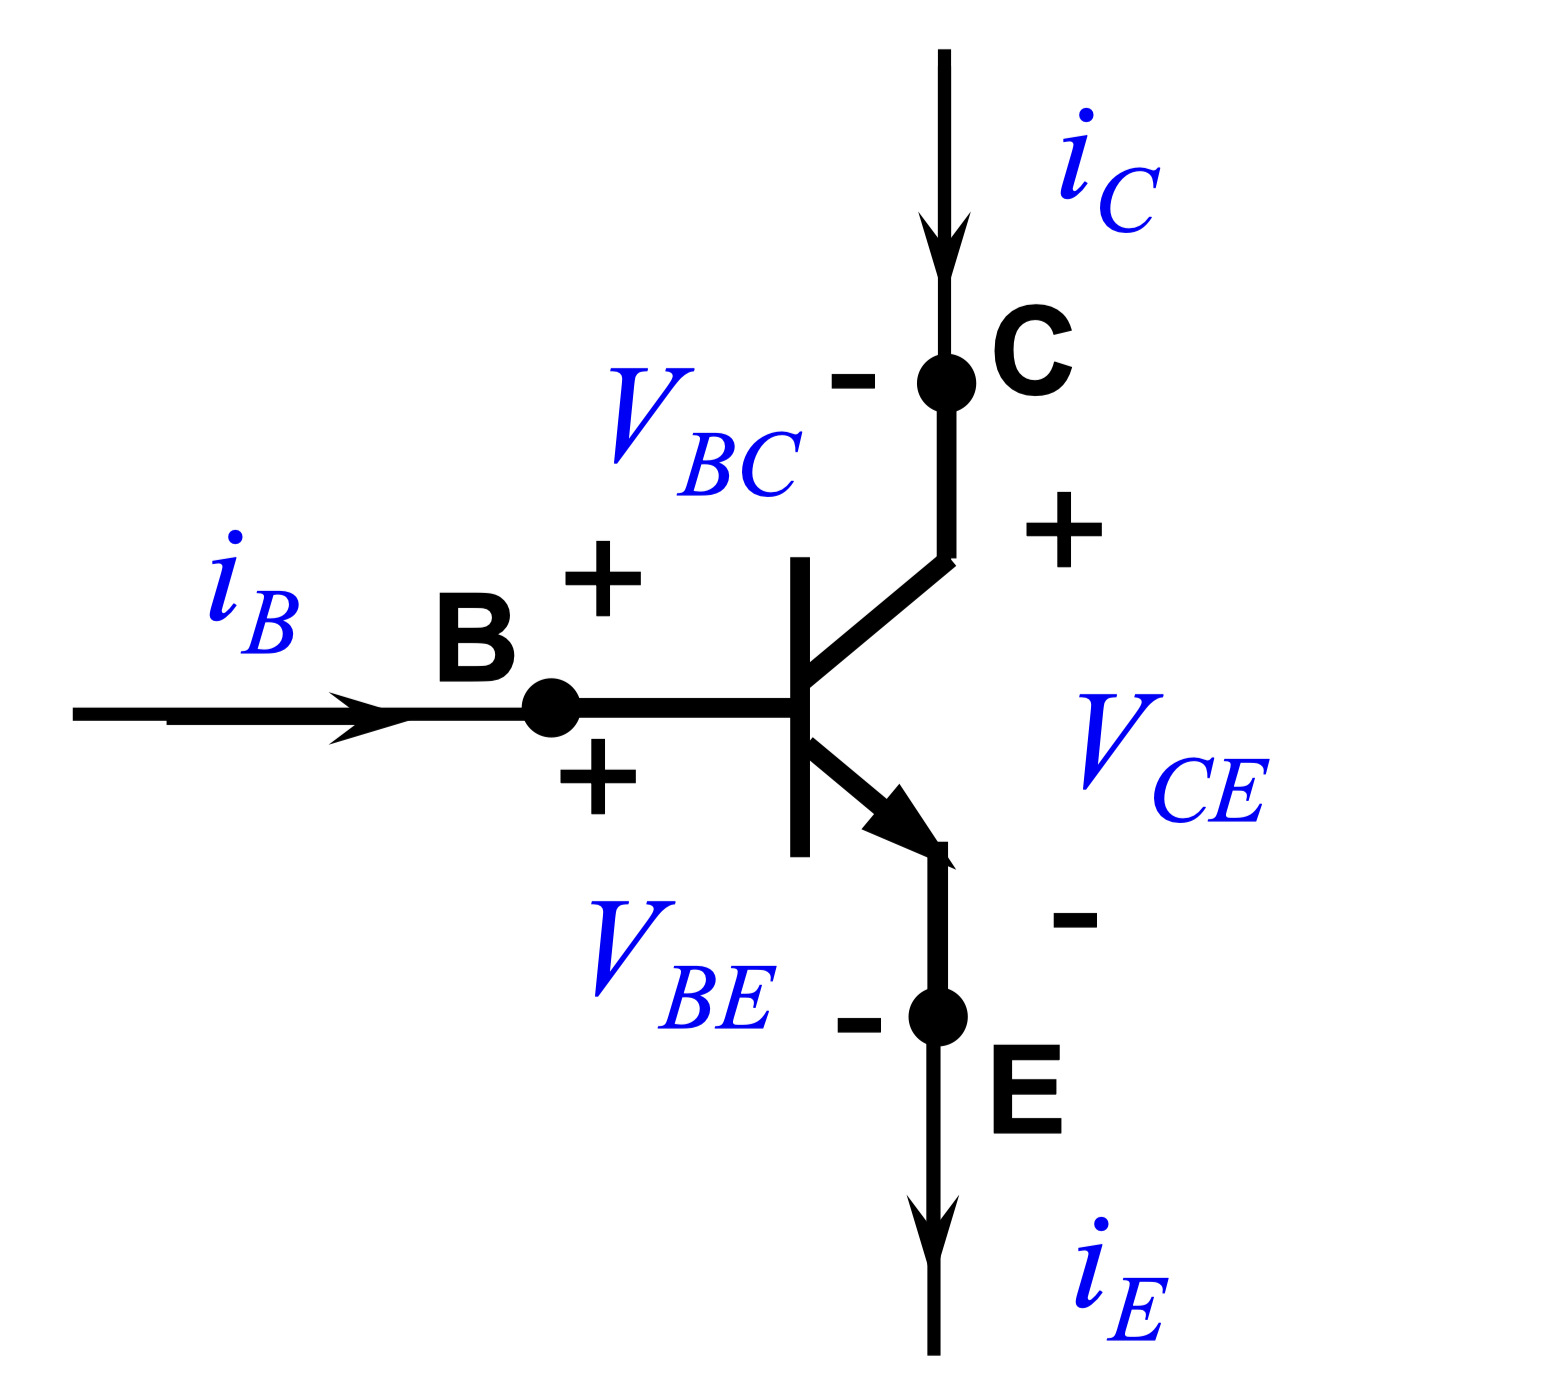
\includegraphics[width=1\linewidth]{image/npnbjt.png}
\end{minipage}
In a non-ideal BJT, there will be \textbf{Early Effect}, meaning $i_C$ is not independent of $V_{BE}$. The $i_C\; v_{CE}$ characteristic will have a slightly upward slope. When you project the slope, there will be a $-V_A$ on the left side of the graph, this is known as the \textbf{Earlt Voltage}.
\begin{figure}[h]
    \centering
    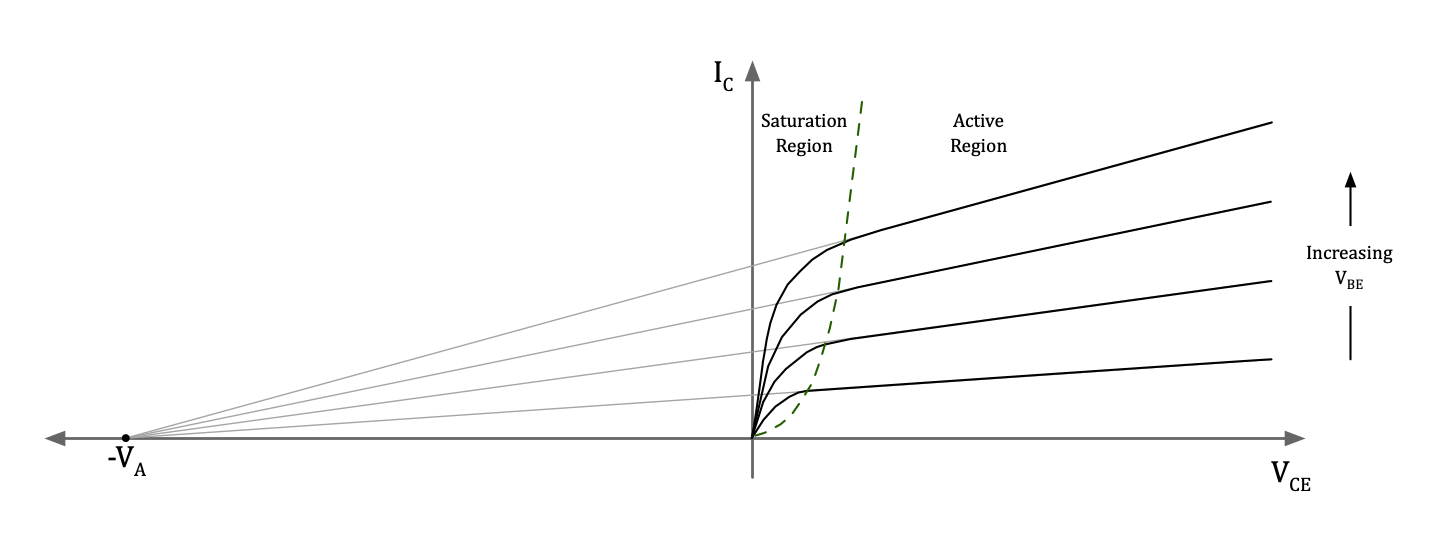
\includegraphics[width=1\linewidth]{image/Earlyeffetc.png}
\end{figure}\\
\textbf{Large-Signal Model and DC analysis}
